%% This source code is under the GNU GPL license version 3
%% Basically : Do what you want as long as you attribute !
%% Steren Giannini (Steren.giannini@gmail.com) 2010

\documentclass[a4paper,11pt]{article} % fonte 11 points, papier a4

\usepackage[francais]{babel}    % faire du franais
\usepackage[utf8]{inputenc}   % accents dans le source
\usepackage[T1]{fontenc}        % accents dans le DVI
\usepackage{graphicx}
\usepackage{multirow}
\usepackage{layout}


%#########
% Commande pour français/anglais,
% changer le #2 pour changer la langue
% #1 = anglais
% #2 = francais
\newcommand{\trad}[2]{#2}
%#########

%#########
% La page
%#########
\pagestyle{empty}               % On ne numrote pas les pages

\setlength{\hoffset}{-1 in}
\setlength{\voffset}{-1 in}
\setlength{\oddsidemargin}{2 cm} 	% Marge gauche sur pages impaires
\setlength{\evensidemargin}{2 cm} 	% Marge gauche sur pages paires
\setlength{\textwidth}{17cm} 	% Largeur de la zone de texte
\trad{
	\setlength{\topmargin}{1cm}    %marge haut
}{
	\setlength{\topmargin}{0,5 cm}
}
\setlength{\headheight}{0pt} 	% Haut de page
\setlength{\headsep}{0pt} 	% Entre le haut de page et le texte
\setlength{\footskip}{0pt} 	% Bas de page + séparation
\setlength{\textheight}{29cm} 	% Hauteur de la zone de texte

%#############################
% Diverses nouvelles commandes
%#############################

% Pour laisser de l'espace entre les lignes du tableau
\newcommand\espace{\vrule height 20pt width 0pt}

% Pour les titres
\newcommand{\titre}[1]{%
	\begin{center}
	%\medskp
	\rule{\textwidth}{1pt}
	\par
	\vspace{0.1cm}
        \textbf{\large #1}
	\par\rule{\textwidth}{1pt}
	\end{center}
	%\medskp
	}
%###################
% Début du document
%###################
\begin{document}

\begin{flushleft}

\trad
{
\begin{tabular}{p{11cm}r}
    %\Large{Steren Giannini} & 8 lotissement Le Moulin\\
    % & 54\,360 Mont sur Meurthe \\
    \Large{Steren Giannini} & 4 rue de la pastorale d'Issy &  \\
    & 92\,130 Issy-Les-Moulineaux \\
    French Student  & France \\
    Date of birth : December 16th 1986  & Tel.: +33 6 84 92 76 24\\
    & E-mail: {steren.giannini@gmail.com}\\
    & \\
    \end{tabular} 
}
{
\begin{tabular}{p{13cm}r}
    \Large{Steren Giannini}  &  \multirow{2}{4cm}{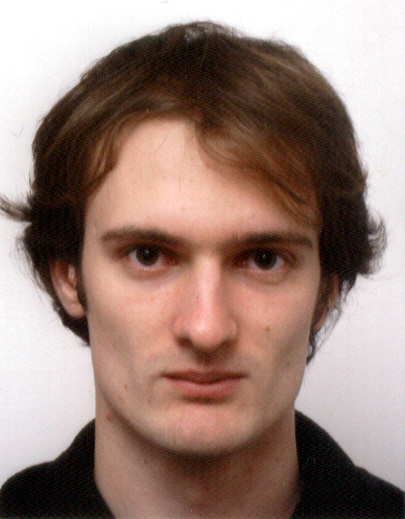
\includegraphics[angle=0, width=3cm]{id_steren_2009.png}}  \\ 
    & \\
    4 rue de la pastorale d'Issy &  \\
    92\,130 Issy-Les-Moulineaux - France & \\
    %8 lotissement Le Moulin &  \\
    %54\,360 Mont sur Meurthe - France & \\
    Tél.: +33 6 84 92 76 24 & \\
    E-mail: {steren.giannini@gmail.com} & \\
    & \\
    Nationalité française & \\
    23 ans & \\
\end{tabular} 
}
\end{flushleft}

%############
% TITLE
%############

%\begin{center}
%\begin{LARGE}
%\textbf{ \textsc{ \trad{TODO}{Recherche poste d'ingénieur} }}
%\end{LARGE}
%\end{center}

%############
\titre{\trad{Education and training}{Etudes}}
%############


\begin{tabular}{cp{0.8\textwidth}}


\textbf{2006-2009}  & \trad{Student at the \textit{\'Ecole Centrale de Lyon}, a French college of general engineering.}
                        {\'Elève-ingénieur à l'\textit{\'Ecole Centrale de Lyon}.} \\
                    & \trad{Third year option: Informatics and Communication}
                        {Option de troisième année : Informatique et Communication, spécialité Multimédia}\\

\espace
\textbf{2004-2006}  & \trad{\textit{Classes préparatoires} of Mathematics and Physics at the \textit{lycée Henri Poincaré} of Nancy.} 
                        {Classes préparatoires au lycée Henri Poincaré à Nancy.} \\ % Mathématiques Supérieures et Mathématiques Spéciales

\espace
\textbf{2004}       & \trad{French \textit{Baccalauréat} (Science) A+ and special english grade.}
                        {Baccalauréat (Série Scientifique) avec mention Très Bien et mention Européenne.} \\ %Anglais

\end{tabular}

\titre{\trad{Employment}{Expérience professionnelle}}
%###################

\begin{tabular}{cp{0.8\textwidth}}
\textbf{2009-2010}							& \trad{Engineer and designer at \textit{Dassault Systèmes}:}{Ingénieur-Designer chez \textit{Dassault Systèmes} :}\\
                                        & \trad{Development of an innovative social platform. -- 1 year}{Développement d'une plateforme innovante de web social  -- 1 an} \\
\espace
\textbf{2009} 							& \trad{End-Of-Course Work at \textit{Dassault Systèmes} (France):}{Travail de Fin d'\'Etude en recherche technologique chez \textit{Dassault Systèmes} :}\\
                                        & \trad{Interactive painting and sculpting on 3D models -- 6 months}{Développement d'une méthode novatrice de peinture et d'ajout de détails sur modèles 3D -- 6 mois} \\
\espace
\textbf{2008-2009} 						& \trad{Software developer working remotely for \textit{Creative Commons}}{Développeur pour \textit{Creative Commons} (travail à distance)} \\
\espace
\textbf{\trad{summer 2008}{été 2008}} 	& \trad{Internship at \textit{Creative Commons} (San Francisco, United States):}{Stage d’application chez \textit{Creative Commons} (San Francisco, \'Etats Unis) :} \\
                                        & \trad{TODO Web development semantic and application prototyping -- 10 weeks}{Développement dans le domaine du web sémantique -- 10 semaines} \\
\espace
\textbf{2008}	                        & \trad{Developer of \textit{Inkscape}, an open source scalable vector graphics editor} {Participation au développement d'\textit{Inkscape}, logiciel libre de dessin vectoriel }\\
%\espace
%\textbf{\trad{july 2007}{juillet 2007}} & \trad{Internship in a team of workers at \textit{Solvay Carbonate France} -- 1 month.}{Stage d’exécution dans une équipe d'ouvriers à \textit{Solvay Carbonate France} -- 1 mois.} \\ %mise en place d’un outil de formation d'un procédé de fabrication.
%\espace
%\textbf{2006-2007} 						& \trad{employee of the \textit{Junior Entreprise} : designing and making dynamic websites.}{réalisateur à la Junior Entreprise de l’École Centrale de Lyon : Conception et réalisation de sites internet dynamiques.} \\
\end{tabular}


\titre{\trad{Competences}{Compétences}}
%#########################

\begin{itemize}
\item \textbf{\trad{Languages}{Langues}}
	\begin{itemize} 
	\trad{\item \textbf{French}, mother tongue}{}
	\item \trad{\textbf{English}, fluent (C1 in the Common European Framework, TOEFL : 603/670)}{\textbf{Anglais}, autonome (niveau C1 du cadre européen de référence, TOEFL : 603/670)}
	\item \trad{\textbf{Spanish}, intermediate (6 years of study)}{\textbf{Espagnol}, niveau intermédiaire (6 années d'études)}
	\item \trad{\textbf{Italian}, intermediate (2 years of study)}{\textbf{Italien}, niveau intermédiaire (2 années d'études)}
	\end{itemize}
\item \textbf{\trad{Computer}{Informatique}}
	\begin{itemize}
	\item \trad{Knowledge of the main office and professional digital art software}             {Maîtrise des principaux outils de bureautique et d'infographie professionnelle}
	\item \trad{Knowledge of programming languages HTML, PHP, Javascript, Java, C++ and Python}            {Expérimenté dans les languages HTML, PHP, Javascript, Java, C++ et Python}
%	\item \trad{Familiar with SVN and Git version control system}                               {Familier avec l'utilisation des systèmes de gestion de versions SVN et Git}
	\item \trad{Everyday use of Linux}                                                          {Utilisation quotidienne d'environnements Linux}
    \item \trad{TODO}                                                                           {Expérience dans l'utilisation de moteurs de rendu temps réel et moteurs physiques}
%	\item \trad{Use of \textit{CATIA} and \textit{Matlab} for the design and regulation of an UAV}{Utilisation des logiciels \textit{CATIA} et \textit{Matlab} dans le cadre d'un projet d'étude}
	\end{itemize}
\end{itemize}

\titre{\trad{Interests}{Centres d'Intérêts}}
%###################

%\begin{itemize}

%\item \textbf{Permis B :} Titulaire du permis B depuis plus de 2 ans.
%\item
    %\textbf{\trad{Spare-time activities}{Loisirs}} 
	\begin{itemize}
	\item \trad{Member of an improvisational theatre company}                   								{Membre d'une troupe d'improvisation théatrale}
	\item \trad{Direction of short films (traditional or computer generated) and other graphical creations}   	{Réalisation de courts métrages et autres créations graphiques} %(traditionnels ou en images de synthèse)
	%\item \trad{Associational life : active member of the student association of the school}					{Vie associative : membre actif de l'association des élèves de l'école}
	%\item \trad{Regular practice of fencing and diving}                         								{Pratique régulière de l'escrime et de la plongée sous-marine}
	\item \trad{Developer of mobile applications for the \textit{Android} OS}  									{Développement d'applications pour mobiles \textit{Android}}
	\item \trad{TODOweb 3d et image}  																			{Suivi de l'actualité des domaines du web et de l'image de synthèse.} 
	\end{itemize}

%\item \textbf{\trad{AFPS:}{AFPS:}} \trad{certificate of first aids training.}{diplomé de l'Attestation de Formation aux Premiers Secours.}
	
%\end{itemize}

%Pour voir les marges :
%\newpage
%\layout

\end{document}
